\section{Methods}
\label{sec:methods}

%------------------------------------------------

The structure of this work is threefold.
First, a dataset of university course descriptions is generated using publicly available data from a number of North American universities.
This process is discussed in \sref{sec:data-acquisition}.
Second, \ac{lda} is applied to the collected data and topics are inferred.
This step is discussed in \sref{sec:topic-modeling}.
Finally, the collected data and inferred topics are presented in a user-facing web application, described in \sref{sec:visualization}.

%------------------------------------------------

\subsection{Data Acquisition}
\label{sec:data-acquisition}

%------------------------------------------------

The primary data manipulated in this study are university catalog course descriptions.
The current experimental data sources are described in \tref{tbl:dataset}.
Note that only Computer Science departments are included in this dataset, in order to simplify the evaluation process and the required number of inferred topics.
Simple web scrapers were written using Python and BeautifulSoup to download publicly available descriptions from university catalogs.
These will be made publicly available at \url{http://github.com/jrouly/trajectory}.
Descriptions and catalog webpages appear in a vast variety of different formats, structures, and HTML correctness, so a parser was written for each university to acquire the unstructured text.
This text was then passed through a cleaning procedure to remove abbreviations and non-English characters, as well as common English stop words.
Finally the text was passed through a stemmer to strip morphology from the words and eliminate duplicate terms.
At the same time, departmental course prerequisite data is collected from the catalog as well.
Prerequisites are limited to courses in the database, meaning that references older courses that are no longer present in the catalog are ignored.
Non-specific prerequisite references (\eg\ \texttt{400-level}) are ignored as well.

%------------------------------------------------

\begin{table}
  \centering
  \begin{tabular}{lcl}
    \toprule
    University & Course Count \\
    \midrule
    American University (AU) & 32 \\
    George Mason University (GMU) & 145 \\
    Kansas State University (KSU) & 83 \\
    Louisiana State University (LSU) & 59 \\
    Portland State University (PDX) & 190 \\
    Rensselaer Polytechnic Institute (RPI) & 61 \\
    University of South Carolina (SC) & 64 \\
    Stanford University (Stanford) & 69 \\
    University of Utah (Utah) & 142 \\
    University of Tennessee, Knoxville (UTK) & 29 \\
    \midrule
    \ac{ec} & 68 \\
    \bottomrule
  \end{tabular}
  \caption{CS program statistics\label{tbl:dataset}}
\end{table}

%------------------------------------------------

The Python scraping framework developed is structured to allow pluggable web scrapers tooled to specific syllabus repositories.
There are a number of existing web scrapers in place pointing to different university course catalogs, but the code can be easily extended in the future to grow the data set.
Integrated in the scraping framework is a lightweight relational database layer to store both course description data and university metadata, including names, URLs, and prerequisite information.
The database layer also stores inferred topics.

%------------------------------------------------

\subsection{Preliminary Data Exploration}
\label{sec:data-exploration}

%------------------------------------------------

In addition to \ac{lda}, other unsupervised machine learning tools can be applied to the same data set.
Simple clustering algorithms (\eg\ K-Means) when given the same bag of words corpus as input act to identify groupings of similar documents according to their term frequency vector Euclidean distance~\cite{lloyd1982}.
Additional, similar clustering algorithms can be applied in a similar manner.

%------------------------------------------------

Preliminary exploratory results are promising.
We applied K-Means clustering to a sample dataset of course descriptions selected from the George Mason University Computer Science online catalog across multiple semesters.
Using course section IDs as ground-truth labels, we clustered the course descriptions.
\tref{table:cluster-metrics} summarizes the metrics computed on the resulting clustering.
Homogeneity represents the ``same-ness'' of a cluster, or the degree to which each cluster contains only members of a single type.
Completeness represents the ``spread'' of courses across clusters, or the degree to which every member of the same type is assigned to the same cluster.
V-Measure is simply the harmonic mean of the prior two metrics.
For each metric, higher is better, and they are bounded from 0 to 1.
A distributed implementation of K-Means available in the Python toolkit \texttt{scikit-learn} was used to perform the clustering.

%------------------------------------------------

The high completeness values are promising: this indicates that many of the same course are assigned under the same cluster prototype.
The low value of homogeneity is unsurprising given the initialization parameters used: K-Means was initialized to detect only 20 clusters, a far smaller number than the magnitude of distinct course sections available.
The number 20 was chosen arbitrarily as a smaller count than the true number of distinct course sections in order to increase cluster size.

%------------------------------------------------

\begin{table}[ht]
\centering
\begin{tabular}{ll}
\toprule
Execution time & 0.144s \\
Homogeneity & 0.415 \\
Completeness & 0.877 \\
V-measure & 0.563 \\
\bottomrule
\end{tabular}
\caption{Preliminary clustering metrics\label{table:cluster-metrics}}
\end{table}

%------------------------------------------------

\subsection{Topic Modeling}
\label{sec:topic-modeling}

After the exploratory clustering process, we pass\-ed clean\-ed data into a topic modeling framework by exporting from the database layer to the filesystem in a structured ``bucket of files'' format.
The Java MALLET library is used to perform \ac{lda} on the course description data.
A data pipeline is constructed using the MALLET API that reads input data, tokenizes it, and trains an \ac{lda} topic model.
The inferred topics are then exported to a common \ac{csv} format and read back into the database layer and applied to existing courses.
Independent runs of \ac{lda} with distinct parameterization are segregated in the database into ``Result Sets'', allowing sets of inferred topics to sit side by side without interfering.
This also allows the presentation of different sets of inferred topics to the end user.

%------------------------------------------------

The initialization parameters of MALLET's \ac{lda} implementation are summarized in \tref{table:lda-parameters}.
Experiments were run varying parameters throughout the experimental range, including the MALLET default values.
However, as the number of topics increased greatly beyond 750, and as $\beta$ decreased greatly below 0.0001, the MALLET framework began to encounter instability and errors.
Any runs which encountered infinite or ``not-a-number'' values were immediately discarded.
Ultimately 77 result sets were retained for analysis.

%------------------------------------------------

\begin{table*}[ht]
\centering
\begin{tabular}{llll}
\toprule
Parameter  & Description & Experimental Range & Default \\
\midrule
$\alpha$   & Dirichlet concentration parameter. & [1, Iterations] & Iterations \\
$\beta$    & Dirichlet concentration parameter. & [0.0001, 0.5] & 0.01 \\
Iterations & The number of \ac{lda} iterations. & --- & 3000 \\
Topics     & The number of topics to infer. & [100, 1000] & --- \\
\bottomrule
\end{tabular}
\caption{LDA Initialization Parameters\label{table:lda-parameters}}
\end{table*}

%------------------------------------------------

\subsection{Visualization}
\label{sec:visualization}

%------------------------------------------------

An interactive, dynamic user visualization of course descriptions and topics has been prototyped.
The visualization is a web-based application built upon the Python Flask library.
The tool interfaces with the same database layer used by the rest of the application framework to provide an aesthetically pleasing user-facing interface with several primary modules.
By default, the web application presents the user with a high level ``dashboard'' overview of the dataset and available result sets, where a result set is the set of topics inferred after a single run of the \ac{lda} module with a distinct initialization set.
After selecting a result set, the user can browse the data by course, department, university, or inferred topics.
The remainder of this section describes implementation details of the tool's primary features.

%------------------------------------------------

\subsubsection{Explore Courses}
\label{sec:vis-course}

%------------------------------------------------

When presented with the complete university dataset, the user may interactively search for a university.
Once a university is selected, the user may search through its registered departments and select a course of interest.
On selecting a course, the text of its description is displayed in both its original format and its cleaned, stemmed format.
Additionally, the course's inferred topics are listed in order of their proportion within the course description.
These topics are expandable, and upon interaction present the user with the list of other known courses with that inferred topic.
Any topics appearing in a document with proportion under 15\% are automatically hidden from the user.
This design choice was implemented to reduce visual clutter from inferred topics with low relevance to the class.

%------------------------------------------------

\subsubsection{Prerequisite Chain Analysis}
\label{sec:vis-prerequisites}

%------------------------------------------------

In addition to the course-specific data, an interactive, collapsible tree visualization of the course' prerequisite chain is displayed.
The recursively generated tree visualization provides a high level view of the course's position within a department.
\fref{fig:prerequisite-detail} details the prerequisite tree visualization.
Above this visualization is the prerequisite chain conceptual analysis tool.
This tool automatically provides a view of any registered prerequisite courses along with their inferred topics.
Any shared topics between the prerequisites and the selected course are highlighted to indicate conceptual overlap.

%------------------------------------------------

Observe the course CS 310 ``Data Structures'' in the upper middle of the prerequisite tree.
\tref{tbl:310-topics} details its topics, along with the topics of its prerequisite courses CS 105 ``Computer Ethics and Society'' and CS 211 ``Object-Oriented Programming''.
Clearly there is a significant area of overlap between a data structures course and an introductory course in object oriented programming, as illustrated by the two italicized overlapping topics.
Specifically, the overlap is in the areas of algorithms and data structures as well as object oriented programming.
The ethics course, however, does not share any conceptual overlap with CS 310.
Inspecting the context of these courses, however, reveals that CS 105 is a common freshman requirement at George Mason, and many upper level classes depend on its completion.
It is intended as a baseline of student maturity rather than a prerequisite because of the concepts it introduces.

%------------------------------------------------

\begin{figure*}
  \centering
  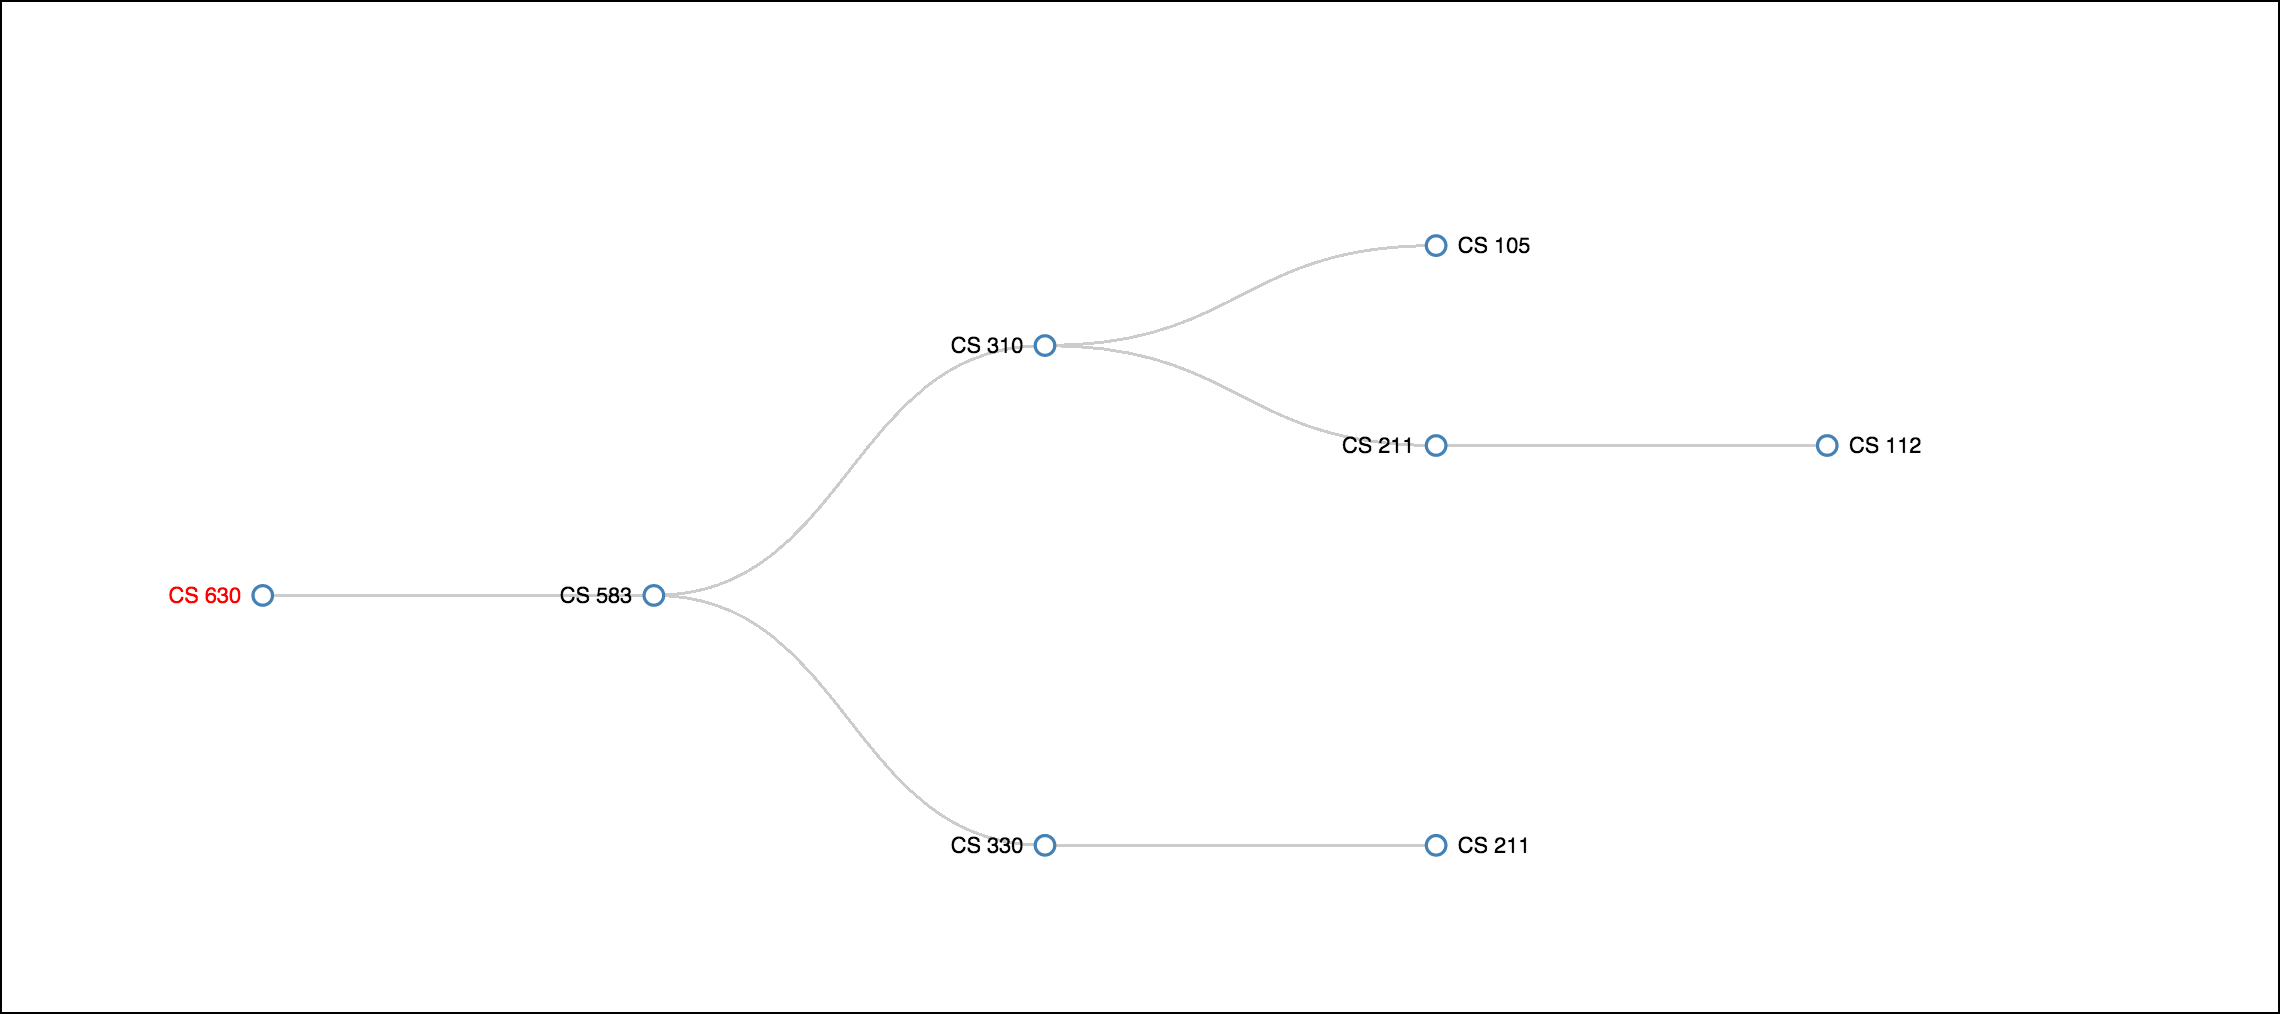
\includegraphics[width=\textwidth]{figures/screenshots/course/prerequisite_detail_cropped.png}
  \caption{Interactive prerequisite tree visualization tool\label{fig:prerequisite-detail}}
\end{figure*}

%------------------------------------------------

\begin{table*}[ht!]
  \centering
  \begin{tabular}{ll}
    \toprule
    GMU CS 310 Topics & Proportion \\
    \midrule
    \emph{languag, object, program, orient, includ, type, abstract, design, implement, concept} & 29.946\% \\
    \emph{program, problem, solv, algorithm, data, structur, comput, introduct, languag, techniqu} & 21.461\% \\
    includ, design, system, topic, comput, introduct, cover, applic, algorithm, techniqu & 26.117\% \\
    \midrule
    GMU CS 211 Topics [Prerequisite] & Proportion \\
    \midrule
    \emph{languag, object, program, orient, includ, type, abstract, design, implement, concept} & 29.433\% \\
    \emph{program, problem, solv, algorithm, data, structur, comput, introduct, languag, techniqu} & 26.772\% \\
    code, compil, pars, analysi, optim, gener, languag, lexic, techniqu, construct & 18.685\% \\
    comput, method, theori, basic, principl, includ, topic, model, cover, scientif & 16.076\% \\
    \midrule
    GMU CS 105 Topics [Prerequisite] & Proportion \\
    \midrule
    ethic, comput, issu, profession, social, technolog, privaci, legal, relat, digit & 75.964\% \\
    \bottomrule
  \end{tabular}
  \caption{Topics of GMU CS 310 and its prerequisite courses, CS 105 and CS 211. Overlapping topics are italicized.\label{tbl:310-topics}}
\end{table*}

%------------------------------------------------

\subsubsection{Compare Departments}
\label{sec:vis-compare}

%------------------------------------------------

The user may also compare two university departments.
Topics inferred from every course in the department are collected and displayed side by side.
Topics unique to each department are displayed separately from the intersection set of common topics.
Similarity metrics describing the relationship between the two departments are defined as well --- Jaccard index, cosine similarity, and Euclidean distance.
Defined as $\frac{\left| A \cap B\right|}{\left| A \cup B\right|}$, the Jaccard index is based on the number of items unique to and shared between each set~\cite{jaccard1912}.
The remaining metrics are based on a ``topic-vector'' representation of each department.
The topic-vector is a binary vector where each bit indicates whether a particular topic was inferred for the given department.
Features are unweighted and the topic-vector indicates only whether a topic is present in a department's topic set, and not its frequency of occurrence.
Interpreting this vector representation geometrically, the Euclidean and cosine distances are calculated.

%------------------------------------------------

\subsubsection{Evaluate Department}
\label{sec:vis-evaluate}

%------------------------------------------------

The tool also allows users to easily evaluate university departments against third party benchmarks.
The \ac{acm} maintains an annual writeup of guidelines for undergraduate computer science education~\cite{CS2013}.
These guidelines include two important sections, the \acf{ec} and Knowledge Areas.
The Knowledge Areas are 18 broad topics within Computer Science as put forth by the \ac{acm}.
\ac{ec} include real course descriptions from disparate sources compiled by the \ac{acm} and manually annotated with the Knowledge Areas they cover.
These data sets are used to perform primary evaluation.
The benchmarks used in this study are the \ac{acm} Knowledge Areas.

%------------------------------------------------

The web tool automatically evaluates the performance of a university department.
The tool checks for conceptual overlap between courses and \ac{acm} Knowledge Areas and predicts Knowledge Area labels where overlap exists.
Additionally, if the department has been manually annotated with Knowledge Areas, these ``ground truth'' labels are compared against the predicted labels, and similarity coefficients between the two sets are computed.
The label set similarity coefficient is computed in two ways.
First, the Jaccard index of the predicted and ground truth labels is calculated.
Then, the percent of the ground truth labels included in the prediction set is calculated.
The web visualization provides an automatic interface for performing this evaluation process.

%------------------------------------------------
